\documentclass[a4paper,14pt]{extarticle}

\usepackage[utf8x]{inputenc}
\usepackage[T1,T2A]{fontenc}
\usepackage[russian]{babel}
\usepackage{hyperref}
\usepackage{indentfirst}
\usepackage{here}
\usepackage{array}
\usepackage{graphicx}
\usepackage{caption}
\usepackage{subcaption}
\usepackage{chngcntr}
\usepackage{amsmath}
\usepackage{amssymb}
\usepackage{pgfplots}
\usepackage{pgfplotstable}
\usepackage[left=2cm,right=2cm,top=2cm,bottom=2cm,bindingoffset=0cm]{geometry}
\usepackage{multicol}
\usepackage{askmaps}
\usepackage{enumitem}

\setitemize{itemsep=0em}
\setenumerate{itemsep=0em}

\renewcommand{\le}{\ensuremath{\leqslant}}
\renewcommand{\leq}{\ensuremath{\leqslant}}
\renewcommand{\ge}{\ensuremath{\geqslant}}
\renewcommand{\geq}{\ensuremath{\geqslant}}
\renewcommand{\epsilon}{\ensuremath{\varepsilon}}
\renewcommand{\phi}{\ensuremath{\varphi}}
\renewcommand{\thefigure}{\arabic{figure}} 	
\renewcommand*\not[1]{\overline{#1}}

%\titleformat*{\section}{\large\bfseries} 
%\titleformat*{\subsection}{\normalsize\bfseries} 
%\titleformat*{\subsubsection}{\normalsize\bfseries} 
%\titleformat*{\paragraph}{\normalsize\bfseries} 
%\titleformat*{\subparagraph}{\normalsize\bfseries} 

\counterwithin{figure}{section}
\counterwithin{equation}{section}
\counterwithin{table}{section}
\newcommand{\sign}[1][5cm]{\makebox[#1]{\hrulefill}}
\graphicspath{{../pics/}}
\captionsetup{justification=centering,margin=1cm}
\def\arraystretch{1.3}
\setlength\parindent{5ex}
%\titlelabel{\thetitle.\quad}

\begin{document}

\begin{titlepage}
\begin{center}
	Санкт-Петербургский Политехнический Университет Петра Великого\\[0.3cm]
	Институт компьютерных наук и технологий \\[0.3cm]
	Кафедра компьютерных систем и программных технологий\\[4cm]
	
	\textbf{ОТЧЕТ}\\ 
	\textbf{по лабораторной работе}\\[0.5cm]
	\textbf{<<Исследование персептронов>>}\\[0.1cm]
	\textbf{Нейроинформатика}\\[4.0cm]
\end{center}

\begin{flushright}
	\begin{minipage}{0.45\textwidth}
		\textbf{Работу выполнил студент}\\[3mm]
		группа 33501/4 \hspace*{10mm} Дьячков В.В.\\[5mm]
		\textbf{Преподаватель}\\[5mm]
		\sign[1.7cm] \hspace*{1mm} к.т.н., доц. Никитин К.В. \\[5mm]
	\end{minipage}
\end{flushright}

\vfill

\begin{center}
	Санкт-Петербург\\
	\the\year
\end{center}
\end{titlepage}

\addtocounter{page}{1}

\tableofcontents
\newpage

\section{Цели работы}

\begin{itemize}
	\item Приобретение навыков построения, инициализации и обучения РФБ-НС.
	\item Исследование РФБ-НС при решении задач аппроксимации статических зависимостей и классификации.
\end{itemize}

\section{Аппроксимация статических зависимостей}

\subsection{Формирование обучающей и тестовой выборки}

%Задайте достаточное для точной аппроксимации количество обучающих примеров (в данном случае совпадающее с числом РБФ-нейронов).

Сформируем обучающую и тестовую выборки на основе ранее созданных функций. На рис. \ref{fig:2_1} изображены сформированные выборки. Исходная выборка из $100$ примеров была разделена на обучающую и тестовую в соотношении $0.7 : 0.3$.

\begin{figure}[H]
\begin{center}
	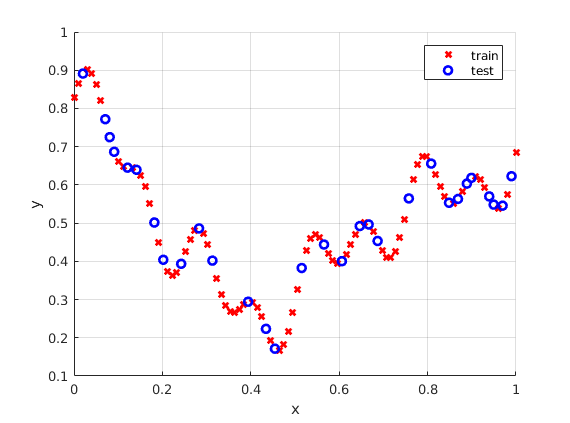
\includegraphics[scale=0.9]{2_1}
	\caption{Обучающая и тестовая выборки}
	\label{fig:2_1}
\end{center}
\end{figure}

\subsection{Аппроксимация с помощью точной РБФ-НС}

%Изменяя ширину РБФ (spread), определите наилучшее значение этого параметра с точки зрения качества аппроксимации. Постройте три графика аппроксимации для разных значений spread: оптимального, больше и меньше оптимального, когда явно видно, что аппроксимация плохая. При построении графиков аппроксимации не забывайте приводить графики исходной желаемой зависимости.
%Постройте график зависимости ошибки аппроксимации от параметра spread в логарифмическом масштабе.
%С помощью точной РБФ-НС (newrbe) аппроксимируйте функцию (для вашего варианта из заданий с номером 5).

Подберем наилучшее значение параметра \code{spread} для обучения с помощью точной РБФ-НС. На рис. \ref{fig:2_2_1} изображена зависимость ошибки \code{perform} от значения параметра \code{spread} в логарифмическом масштабе. 
\begin{figure}[H]
\begin{center}
	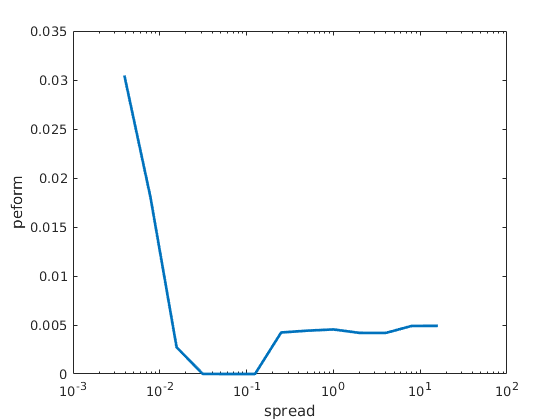
\includegraphics[scale=0.9]{2_2_1}
	\caption{Зависимость \code{perform} от \code{spread}}
	\label{fig:2_2_1}
\end{center}
\end{figure}

Оптимальным можно считать значения \code{spread} $\approx 0.1$. При таком значении параметра ошибка аппроксимации $\sim 10^{-20}$. Построим два графика аппроксимации для оптимального значения \code{spread} и больше оптимального. При уменьшении параметра даже до $10^{-10}$ функция аппроксимируется практически без ошибок. На рис. \ref{fig:2_2_2} изображены построенные аппроксимации.
\begin{figure}[H]
\begin{center}
	\begin{subfigure}{0.49\textwidth}
		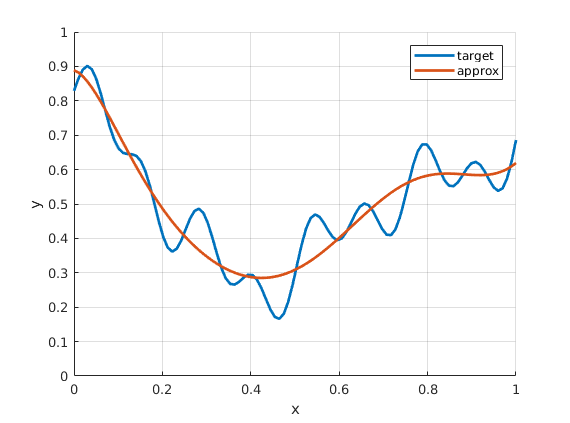
\includegraphics[width=\textwidth]{2_2_2}
		\caption{\code{spread = 1}}
	\end{subfigure}
	\begin{subfigure}{0.49\textwidth}
		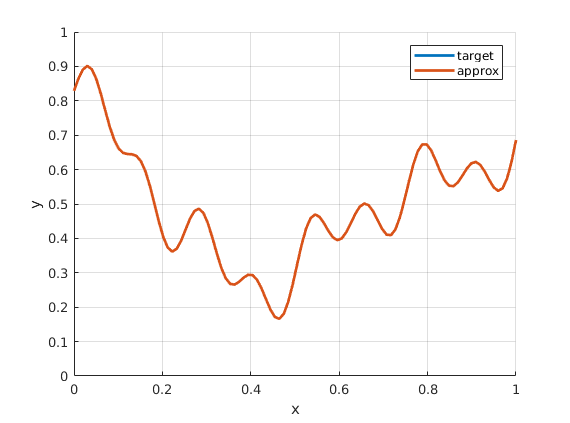
\includegraphics[width=\textwidth]{2_2_3}
		\caption{\code{spread = 0.1}}
	\end{subfigure}
	\caption{Аппроксимация при разных значениях \code{spread}}
	\label{fig:2_2_2}
\end{center}
\end{figure}

\subsection{Аппроксимация с помощью приближенной РБФ-НС}

%Изменяя значение допустимой ошибки (goal), постройте зависимость числа используемых РБФ-нейронов от допустимой ошибки аппроксимации. Для промежуточных результатов постройте графики аппроксимации.

На рис. \ref{fig:2_3_1} изображена зависимость числа используемых РБФ-нейронов от допустимой ошибки аппроксимации \code{goal} в логарифмическом масштабе.
\begin{figure}[H]
\begin{center}
	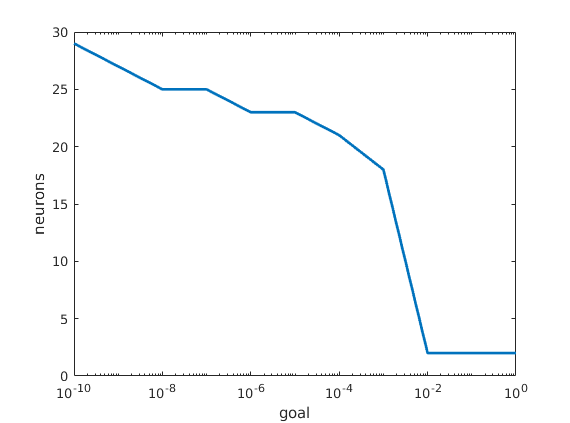
\includegraphics[scale=0.9]{2_3_1}
	\caption{Зависимость числа нейронов от \code{goal}}
	\label{fig:2_3_1}
\end{center}
\end{figure}

На рис. \ref{fig:2_3_2} изображены аппроксимации при разных значениях допустимой ошибки.
\begin{figure}[H]
\begin{center}
	\begin{subfigure}{0.49\textwidth}
		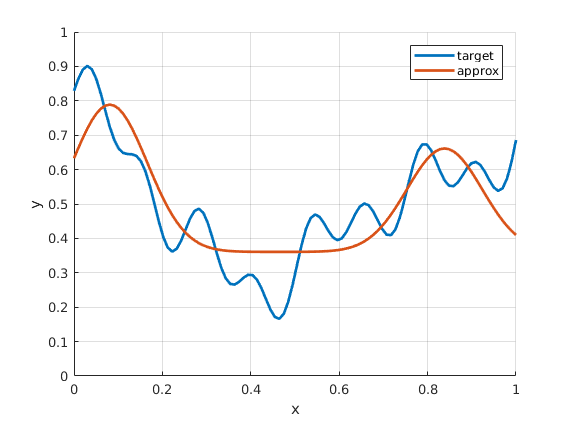
\includegraphics[width=\textwidth]{2_3_2}
		\caption{\code{goal = 0.01} (2 нейрона)}
	\end{subfigure}
	\begin{subfigure}{0.49\textwidth}
		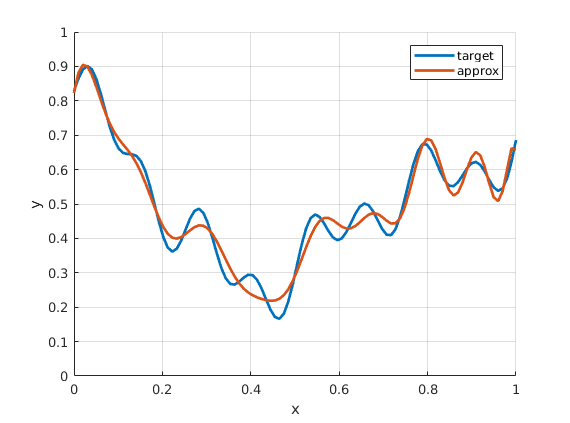
\includegraphics[width=\textwidth]{2_3_3}
		\caption{\code{goal = 0.001} (18 нейронов)}
	\end{subfigure}
\end{center}
\end{figure}
\begin{figure}[H]
\begin{center}
	\begin{subfigure}{0.49\textwidth}
		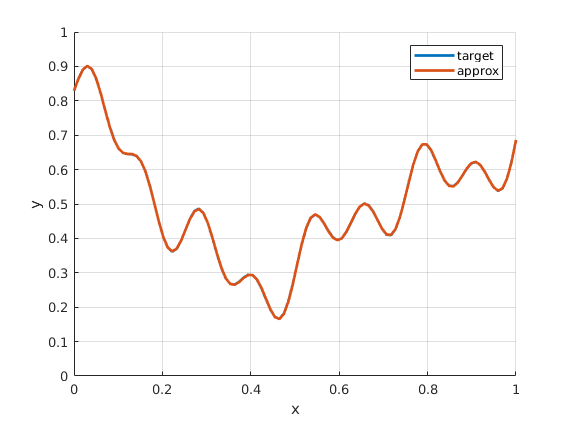
\includegraphics[width=\textwidth]{2_3_4}
		\caption*{(c) \code{goal = 0.0001} (23 нейрона)}
	\end{subfigure}
	\caption{Аппроксимация при разных значениях \code{goal}}
	\label{fig:2_3_2}
\end{center}
\end{figure}

\subsection{Аппроксимация с помощью GRNN}

%По аналогии с newrb изменяя ширину РБФ (spread), определите наилучшее значение этого параметра с точки зрения качества аппроксимации. Постройте график аппроксимации на исходной зависимости.
%Уменьшите объем обучающей выборки в несколько раз (рассмотрите 3 случая) и подберите оптимальные значения параметра spread для каждого случая. Постройте полученные графики аппроксимации. Приведите значения ошибок.

Подберем наилучшее значение параметра \code{spread} для обучения с помощью GRNN. На рис. \ref{fig:2_4_1} изображена зависимость ошибки \code{perform} от значения параметра \code{spread} в логарифмическом масштабе. 
\begin{figure}[H]
\begin{center}
	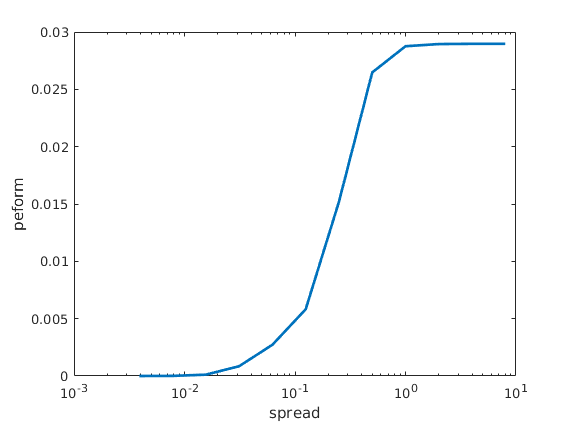
\includegraphics[scale=0.9]{2_4_1}
	\caption{Зависимость \code{perform} от \code{spread}}
	\label{fig:2_4_1}
\end{center}
\end{figure}

Оптимальным можно считать значения \code{spread} $\leq 0.01$. В отличии от точной РБФ-НН, при задании параметра \code{spread} меньшим, чем оптимальное значение, ошибка аппроксимации не увеличивается. Построим два графика аппроксимации для оптимального значения \code{spread} и больше оптимального. При уменьшении параметра даже до $10^{-10}$ функция аппроксимируется без ошибок. На рис. \ref{fig:2_4_2} изображены построенные аппроксимации.
\begin{figure}[H]
\begin{center}
	\begin{subfigure}{0.49\textwidth}
		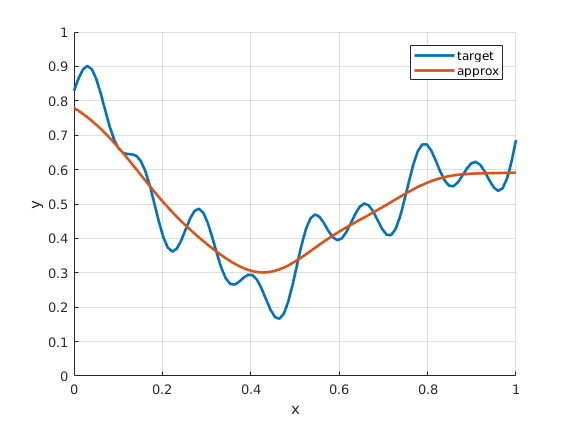
\includegraphics[width=\textwidth]{2_4_2}
		\caption{\code{spread = 0.1}}
	\end{subfigure}
	\begin{subfigure}{0.49\textwidth}
		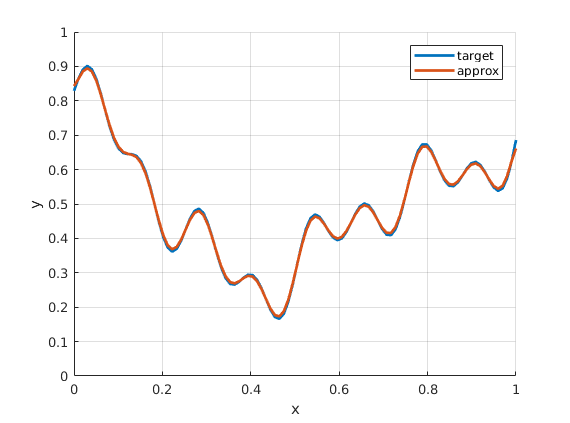
\includegraphics[width=\textwidth]{2_4_3}
		\caption{\code{spread = 0.01}}
	\end{subfigure}
	\caption{Аппроксимация при разных значениях \code{spread}}
	\label{fig:2_4_2}
\end{center}
\end{figure}

\subsection{Сравнение качества апрпоксимации}

%Сравните качество аппроксимации сетями прямого распространения и различными вариантами РБФ-НС (точной, приближенной РБФ-НС и GRNN) по различным показателям:
%- число нейронов, требуемое для достижения заданного качества аппроксимации;
%- время обучения;
%- сложность настройки (выбора параметров) НС.
%Постройте на одном графике зависимости ошибки от числа нейронов для различных типов НС.

По сравнению с сетями прямого распространения, РБФ сети могут добиться в разы более низкой ошибки аппроксимации: $\sim 10^{-20}$ против $\sim 10^{-6}$. Однако, в точной РБС-НС и GRNN количество нейронов равняется числу примеров в обучающей выборке, в то время как в НСПР требуется около $20 \div 30$ нейронов для аппроксимации данной зависимости. В приближенной РБФ-НС количество используемых нейронов напрямую зависит от допустимой ошибки: для допустимой ошибки $\sim 10^{-2}$ требуется всего 2 нейрона, для $\sim 10^{-5}$ около 20, а для $\sim 10^{-10}$ все 100 нейронов, что соответствует размеру выборки. РБФ-НС имеют сложности в настройке, так как от выбора параметров \code{spread} и \code{goal} напрямую зависит качество аппроксимации, однако и НСПР имеют свои сложности:  необходимо задавать количество нейронов скрытого слоя и параметры функции обучения.

\section{Разбиение плоскости на $2$ класса}

\subsection{Формирование обучающей и тестовой выборки}

%Задайте достаточное для точной классификации количество обучающих примеров.

Сформируем обучающую и тестовую выборки на основе ранее созданных функций. На рис. \ref{fig:3_1} изображены сформированные выборки.
\begin{figure}[H]
\begin{center}
	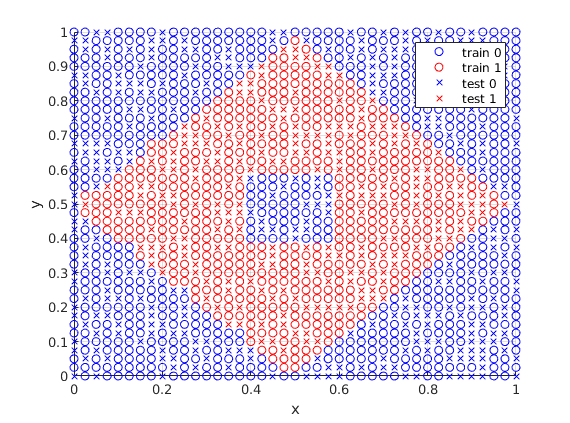
\includegraphics[scale=1]{3_1}
	\caption{Обучающая и тестовая выборки}
	\label{fig:3_1}
\end{center}
\end{figure}

\subsection{Подбор значения spread}

%Подберите оптимальное значение spread в смысле минимальной ошибки на тестовой выборке. Визуализируйте результаты классификации (диаграмма соотнесения тестовых примеров с классами, раскраска плоскости). Приведите значение средней ошибки.
%Постройте дополнительно графики классификации для значений spread, больших и меньших оптимального, когда явно видно, что классификация неудовлетворительная.

Подберем наилучшее значение параметра \code{spread} для обучения с помощью точной РБФ-НС. На рис. \ref{fig:3_2_1} изображена зависимость ошибки \code{perform} от значения параметра \code{spread} в логарифмическом масштабе. 
\begin{figure}[H]
\begin{center}
	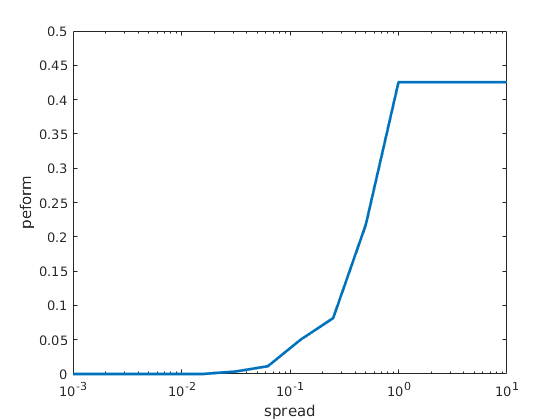
\includegraphics[scale=0.75]{3_2_1}
	\caption{Зависимость \code{perform} от \code{spread}}
	\label{fig:3_2_1}
\end{center}
\end{figure}

Оптимальным можно считать значения \code{spread} $\leq 0.01$. При таком значении параметра ошибка классификации равна нулю. Построим три графика классификации: для оптимального значения \code{spread}, большего и меньшего, чем оптимальное. На рис. \ref{fig:3_2_2} -- \ref{fig:3_2_4} изображены построенные классификации и матрицы неточностей для тестовой выборки.
\begin{figure}[H]
\begin{center}
	\begin{subfigure}{0.49\textwidth}
		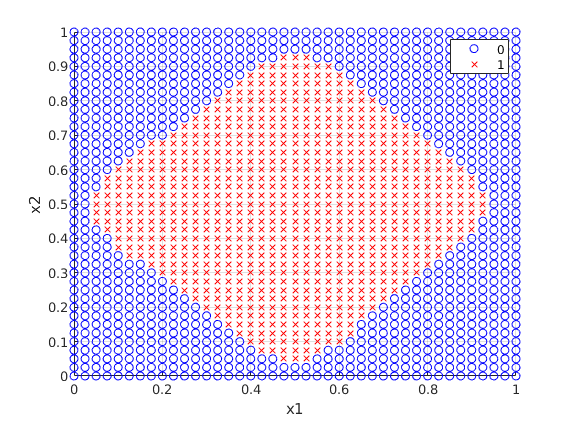
\includegraphics[width=\textwidth]{3_2_2}
		\caption{Классификация}
	\end{subfigure}
	\begin{subfigure}{0.49\textwidth}
		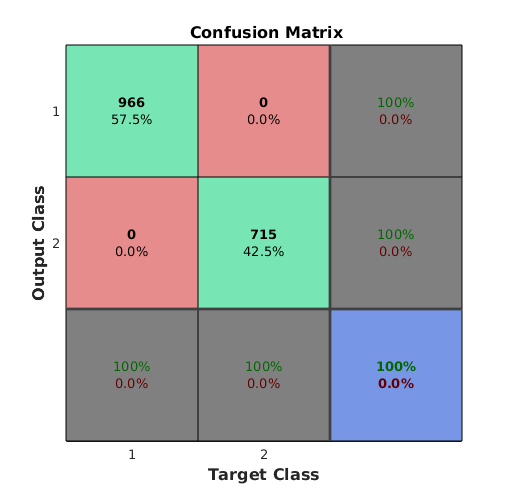
\includegraphics[width=\textwidth]{3_2_5}
		\caption{Матрица неточностей}
	\end{subfigure}
	\caption{Классификация и матрица неточностей при \code{spread = 0.2}}
	\label{fig:3_2_2}
\end{center}
\end{figure}

\begin{figure}[H]
\begin{center}
	\begin{subfigure}{0.49\textwidth}
		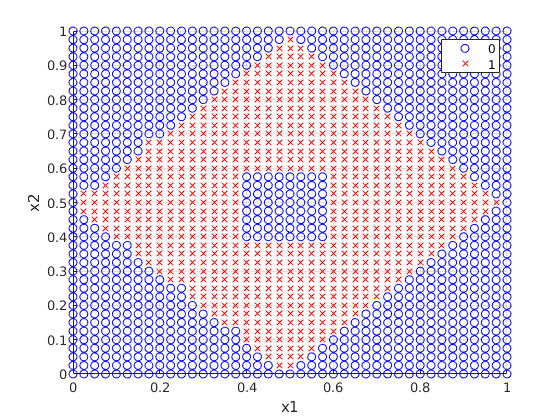
\includegraphics[width=\textwidth]{3_2_3}
		\caption{Классификация}
	\end{subfigure}
	\begin{subfigure}{0.49\textwidth}
		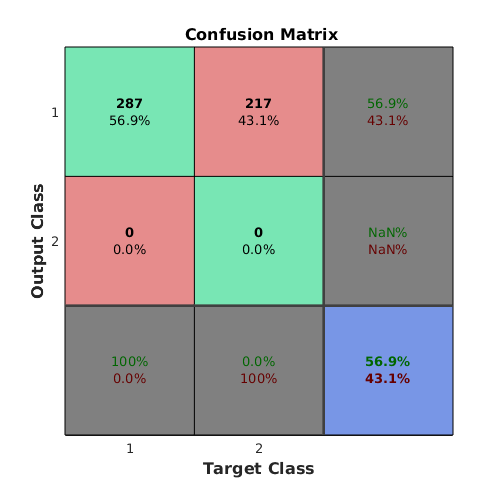
\includegraphics[width=\textwidth]{3_2_6}
		\caption{Матрица неточностей}
	\end{subfigure}
	\caption{Классификация и матрица неточностей при \code{spread = 0.0001}}
	\label{fig:3_2_3}
\end{center}
\end{figure}


\begin{figure}[H]
\begin{center}
	\begin{subfigure}{0.49\textwidth}
		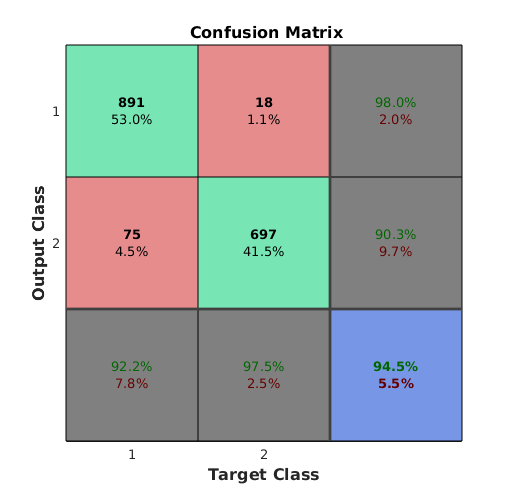
\includegraphics[width=\textwidth]{3_2_4}
		\caption{Классификация}
	\end{subfigure}
	\begin{subfigure}{0.49\textwidth}
		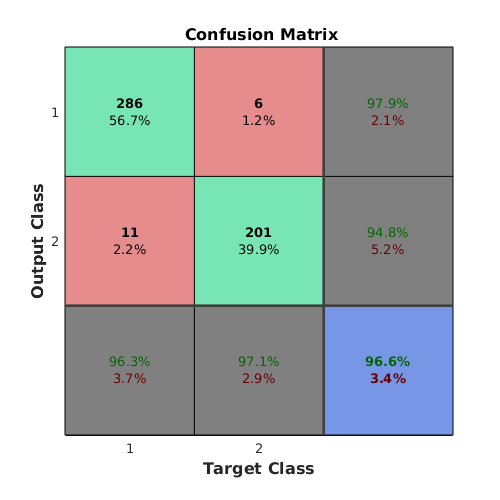
\includegraphics[width=\textwidth]{3_2_7}
		\caption{Матрица неточностей}
	\end{subfigure}
	\caption{Классификация и матрица неточностей при \code{spread = 0.01}}
	\label{fig:3_2_4}
\end{center}
\end{figure}


\subsection{Уменьшение объема выборки}

%Уменьшите объем обучающей выборки в несколько раз (рассмотрите 3 случая) и подберите оптимальные значения параметра spread для каждого случая. Визуализируйте результаты классификации и приведите значение средней ошибки.

Уменьшим обучающую выборку в 5 раз, т.е. с 1681 примера до 336. На рис. \ref{fig:3_3_1} приведена зависимость ошибки \code{perform} от значения параметра \code{spread} в логарифмическом масштабе. 
\vspace{-0.5cm}
\begin{figure}[H]
\begin{center}
	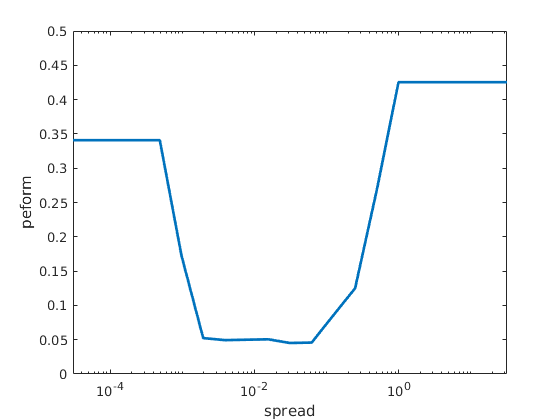
\includegraphics[scale=0.75]{3_3_1}
	\caption{Зависимость \code{perform} от \code{spread}}
	\label{fig:3_3_1}
\end{center}
\end{figure}
\vspace{-0.5cm}

Оптимальным можно считать \code{spread = 0.01}, средняя ошибка равна $0.0553$. Для данного значения классифицируем выборку всех входных значений. На рис. \ref{fig:3_3_2} приведены результаты классификации и матрица неточностей при \code{spread = 0.01}.
\vspace{-1cm}
\begin{figure}[H]
\begin{center}
	\begin{subfigure}{0.49\textwidth}
		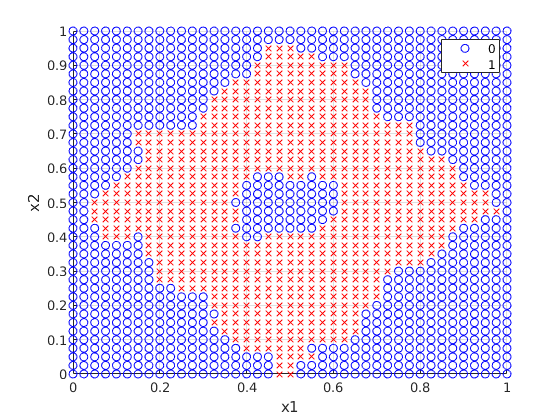
\includegraphics[width=\textwidth]{3_3_2}
		\caption{Классификация}
	\end{subfigure}
	\begin{subfigure}{0.47\textwidth}
		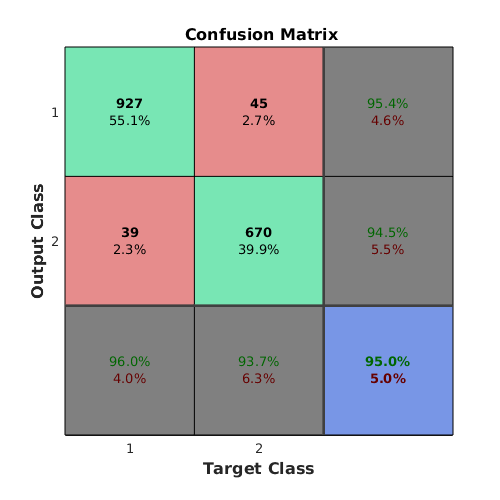
\includegraphics[width=\textwidth]{3_3_3}
		\caption{Матрица неточностей}
	\end{subfigure}
	\caption{Классификация и матрица неточностей при \code{spread = 0.01}}
	\label{fig:3_3_2}
\end{center}
\end{figure}

Уменьшим обучающую выборку в 10 раз, т.е. с 1681 примера до 168. На рис. \ref{fig:3_3_4} приведена зависимость ошибки \code{perform} от значения параметра \code{spread} в логарифмическом масштабе.
\vspace{-0.5cm} 
\begin{figure}[H]
\begin{center}
	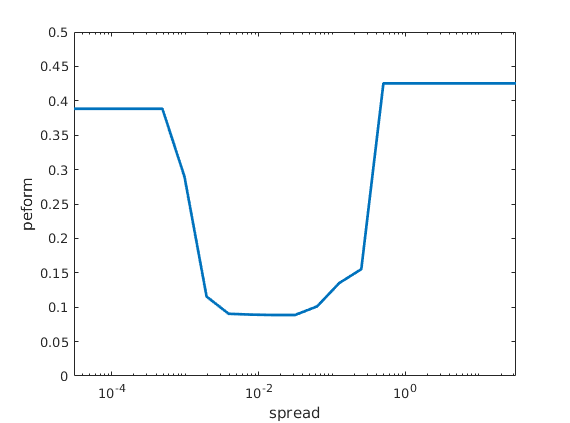
\includegraphics[scale=0.75]{3_3_4}
	\caption{Зависимость \code{perform} от \code{spread}}
	\label{fig:3_3_4}
\end{center}
\end{figure}
\vspace{-0.5cm}

Оптимальным можно также считать \code{spread = 0.01}. Средняя ошибка равна $0.0744$. Для данного значения классифицируем выборку всех входных значений. На рис. \ref{fig:3_3_5} приведены результаты классификации и матрица неточностей при \code{spread = 0.01}.
\vspace{-0.5cm}
\begin{figure}[H]
\begin{center}
	\begin{subfigure}{0.49\textwidth}
		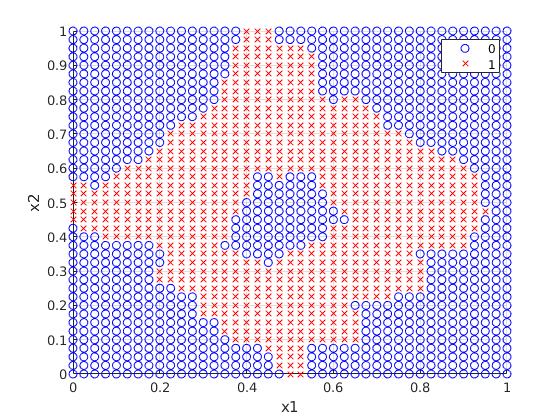
\includegraphics[width=\textwidth]{3_3_5}
		\caption{Классификация}
	\end{subfigure}
	\begin{subfigure}{0.47\textwidth}
		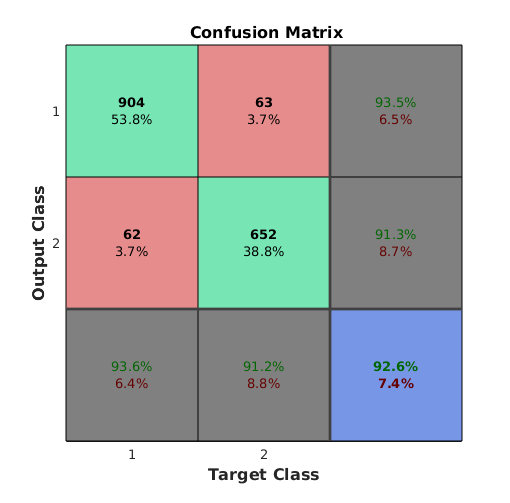
\includegraphics[width=\textwidth]{3_3_6}
		\caption{Матрица неточностей}
	\end{subfigure}
	\caption{Классификация и матрица неточностей при \code{spread = 0.01}}
	\label{fig:3_3_5}
\end{center}
\end{figure}

\subsection{Сравнение качества классификации}

%Постройте поверхность ошибки в плоскости двух параметров: ширина РБФ-функции spread и объем обучающей выборки.
%Сравните полученные результаты с НС прямого распространения по аналогии с п. 3 задания 1.

По сравнению с сетями прямого распространения, PNN смогла добиться нулевой ошибки, в то время как НСПР лишь $\sim 10^{-4}$. Однако, в PNN количество нейронов равняется обучающей выборке ($1681$ нейрон), в то время как в НСПР требовалось около $20 \div 30$ нейронов для данной классификации. PNN оказалось проще настроить, так как необходимо задать только один параметр \code{spread}. В НСПР же необходимо задавать количество нейронов скрытого слоя и параметры функции обучения.

\section{Разбиение плоскости на $N$ классов}

\subsection{Формирование обучающей и тестовой выборки}

Сформируем обучающую и тестовую выборки на основе ранее созданных функций. На рис. \ref{fig:4_1} изображены сформированные выборки: обучающая выборка обозначена ноликами, а тестовая -- крестиками.
\begin{figure}[H]
\begin{center}
	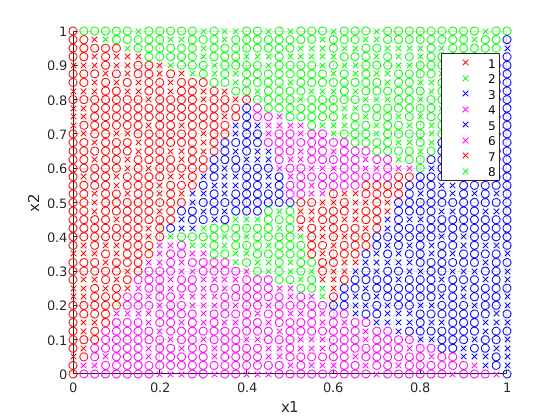
\includegraphics[scale=1]{4_1}
	\caption{Обучающая и тестовая выборки}
	\label{fig:4_1}
\end{center}
\end{figure}

\subsection{Подбор значения spread}

%Подберите оптимальное значение spread в смысле минимальной ошибки на тестовой выборке. Визуализируйте результаты классификации (диаграмма соотнесения тестовых примеров с классами, раскраска плоскости). Приведите значение средней ошибки.
%Постройте дополнительно графики классификации для значений spread, больших и меньших оптимального, когда явно видно, что классификация неудовлетворительная.
%Дополнительно приведите матрицы неточностей и рассчитайте ошибки первого и второго родов.

Подберем наилучшее значение параметра \code{spread} для обучения с помощью точной РБФ-НС. На рис. \ref{fig:4_2_1} изображена зависимость ошибки \code{perform} от значения параметра \code{spread} в логарифмическом масштабе. 
\vspace{-1cm}
\begin{figure}[H]
\begin{center}
	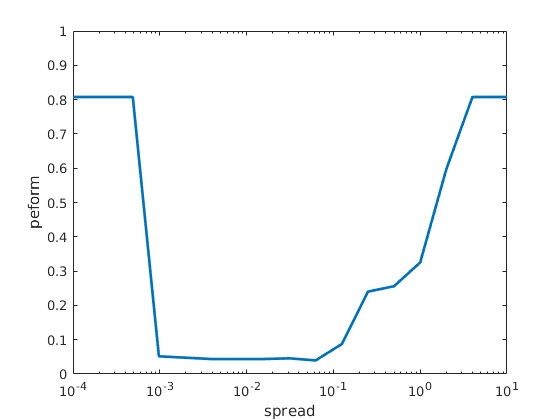
\includegraphics[scale=0.75]{4_2_1}
	\caption{Зависимость \code{perform} от \code{spread}}
	\label{fig:4_2_1}
\end{center}
\end{figure}
\vspace{-0.5cm}

Оптимальным можно считать значения \code{spread} $\approx 0.01$. При таком значении ошибка классификации на тестовой выборке равна 0.0496. Построим три графика классификации: для оптимального значения \code{spread}, большего и меньшего, чем оптимальное. На рис. \ref{fig:3_2_2} -- \ref{fig:3_2_4} изображены построенные классификации и матрицы неточностей для тестовой выборки. 
\vspace{-1cm}
\begin{figure}[H]
\begin{center}
	\begin{subfigure}{0.49\textwidth}
		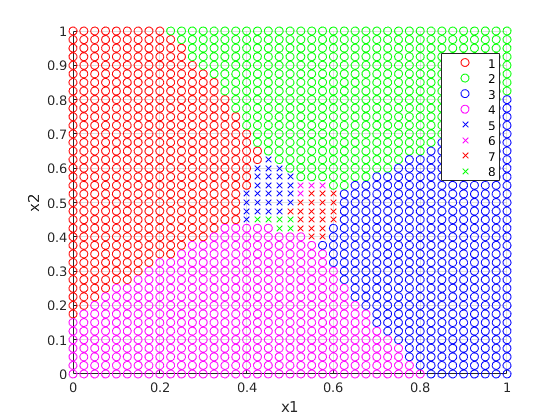
\includegraphics[width=\textwidth]{4_3_1}
		\caption{Классификация}
	\end{subfigure}
	\begin{subfigure}{0.47\textwidth}
		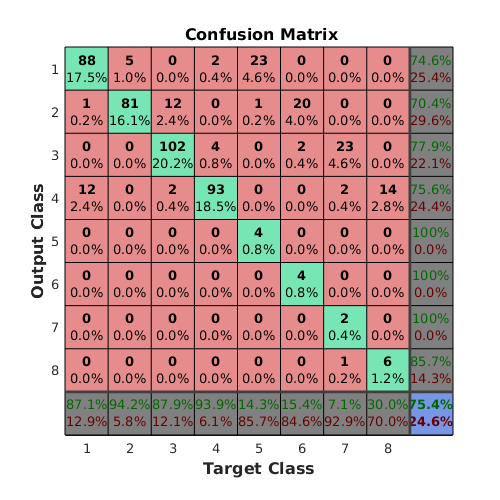
\includegraphics[width=\textwidth]{4_3_4}
		\caption{Матрица неточностей}
	\end{subfigure}
	\caption{Классификация и матрица неточностей при \code{spread = 0.2}}
	\label{fig:3_2_4}
\end{center}
\end{figure}

\begin{figure}[H]
\begin{center}
	\begin{subfigure}{0.49\textwidth}
		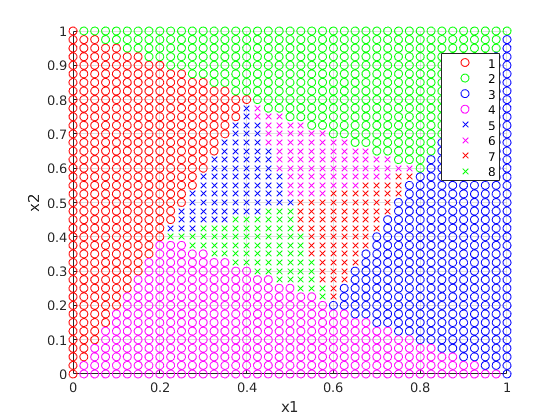
\includegraphics[width=\textwidth]{4_3_2}
		\caption{Классификация}
	\end{subfigure}
	\begin{subfigure}{0.49\textwidth}
		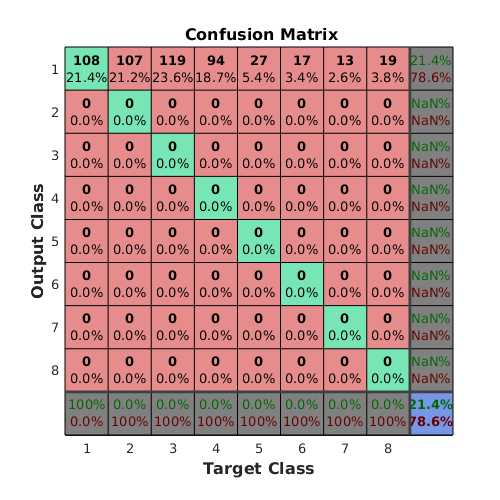
\includegraphics[width=\textwidth]{4_3_5}
		\caption{Матрица неточностей}
	\end{subfigure}
	\caption{Классификация и матрица неточностей при \code{spread = 0.0001}}
	\label{fig:3_2_4}
\end{center}
\end{figure}

\begin{figure}[H]
\begin{center}
	\begin{subfigure}{0.49\textwidth}
		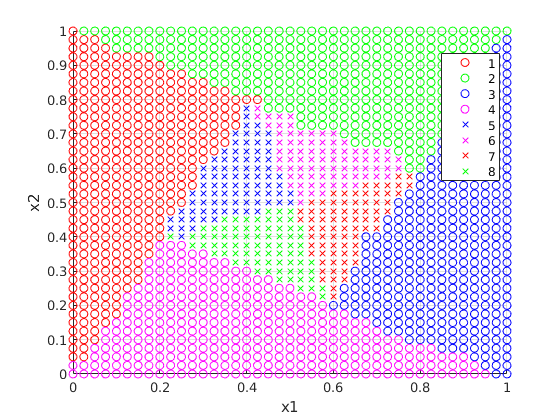
\includegraphics[width=\textwidth]{4_3_3}
		\caption{Классификация}
	\end{subfigure}
	\begin{subfigure}{0.49\textwidth}
		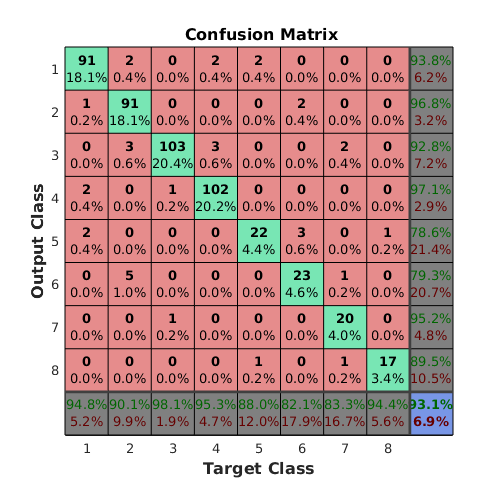
\includegraphics[width=\textwidth]{4_3_6}
		\caption{Матрица неточностей}
	\end{subfigure}
	\caption{Классификация и матрица неточностей при \code{spread = 0.01}}
	\label{fig:3_2_4}
\end{center}
\end{figure}

\subsection{Уменьшение объема выборки}

%Уменьшите объем обучающей выборки в несколько раз (рассмотрите 3 случая) и подберите оптимальные значения параметра spread для каждого случая. Визуализируйте результаты классификации и приведите значение средней ошибки.

Уменьшим обучающую выборку в 5 раз, т.е. с 1681 примера до 336. На рис. \ref{fig:4_4_1} приведена зависимость ошибки \code{perform} от значения параметра \code{spread} в логарифмическом масштабе. 
\vspace{-0.5cm}
\begin{figure}[H]
\begin{center}
	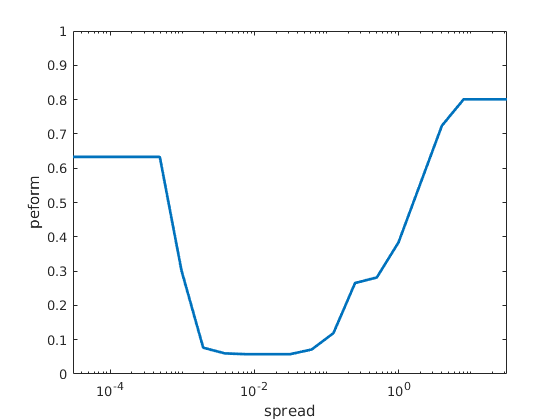
\includegraphics[scale=0.75]{4_4_1}
	\caption{Зависимость \code{perform} от \code{spread}}
	\label{fig:4_4_1}
\end{center}
\end{figure}
\vspace{-0.5cm}

Оптимальным можно считать \code{spread = 0.01}, средняя ошибка равна $0.6098$. Для данного значения классифицируем выборку всех входных значений. На рис. \ref{fig:4_4_2} приведены результаты классификации и матрица неточностей при \code{spread = 0.01}.
\vspace{-1cm}
\begin{figure}[H]
\begin{center}
	\begin{subfigure}{0.49\textwidth}
		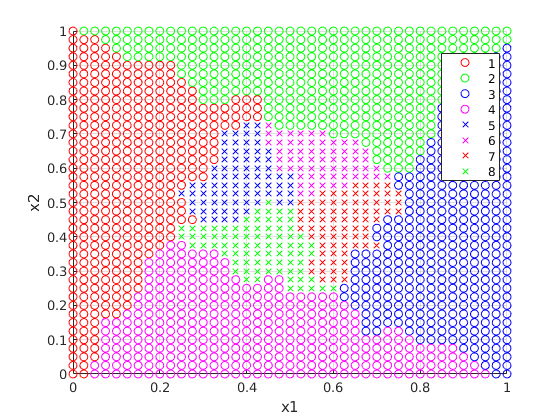
\includegraphics[width=\textwidth]{4_4_2}
		\caption{Классификация}
	\end{subfigure}
	\begin{subfigure}{0.47\textwidth}
		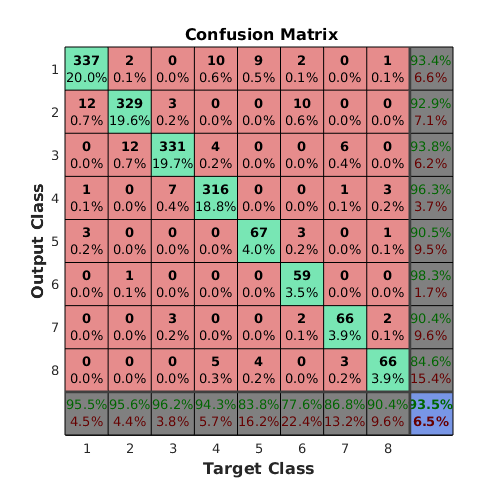
\includegraphics[width=\textwidth]{4_4_3}
		\caption{Матрица неточностей}
	\end{subfigure}
	\caption{Классификация и матрица неточностей при \code{spread = 0.01}}
	\label{fig:4_4_2}
\end{center}
\end{figure}

Уменьшим обучающую выборку в 10 раз, т.е. с 1681 примера до 168. На рис. \ref{fig:4_4_4} приведена зависимость ошибки \code{perform} от значения параметра \code{spread} в логарифмическом масштабе.
\vspace{-0.5cm} 
\begin{figure}[H]
\begin{center}
	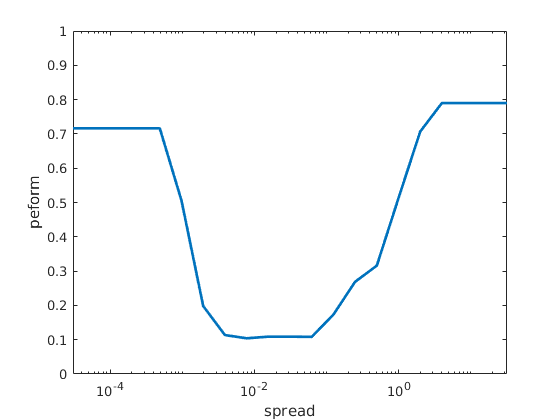
\includegraphics[scale=0.75]{4_4_4}
	\caption{Зависимость \code{perform} от \code{spread}}
	\label{fig:4_4_4}
\end{center}
\end{figure}
\vspace{-0.5cm}

Оптимальным можно также считать \code{spread = 0.01}. Средняя ошибка равна $1.0196$. Для данного значения классифицируем выборку всех входных значений. На рис. \ref{fig:4_4_5} приведены результаты классификации и матрица неточностей при \code{spread = 0.01}.
\vspace{-1cm}
\begin{figure}[H]
\begin{center}
	\begin{subfigure}{0.49\textwidth}
		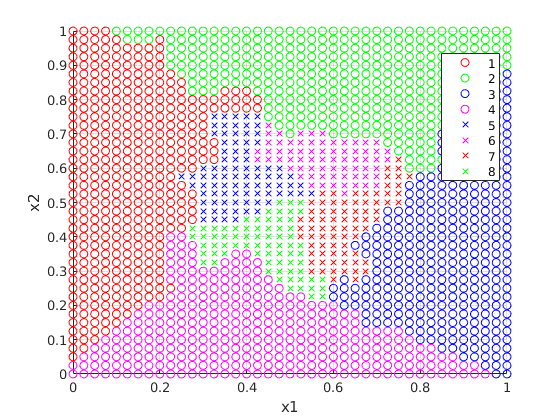
\includegraphics[width=\textwidth]{4_4_5}
		\caption{Классификация}
	\end{subfigure}
	\begin{subfigure}{0.49\textwidth}
		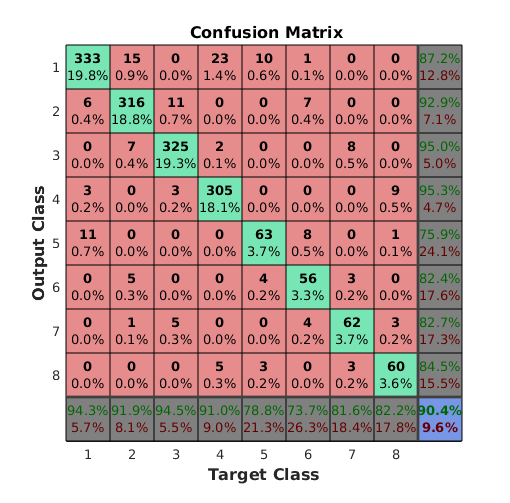
\includegraphics[width=\textwidth]{4_4_6}
		\caption{Матрица неточностей}
	\end{subfigure}
	\caption{Классификация и матрица неточностей при \code{spread = 0.01}}
	\label{fig:4_4_5}
\end{center}
\end{figure}

\vspace{-1cm}
\subsection{Сравнение качества классификации}

%Постройте поверхность ошибки в плоскости двух параметров: ширина РБФ-функции spread и объем обучающей выборки.
%Сравните полученные результаты с НС прямого распространения по аналогии с п. 3 задания 1.

Построим зависимость ошибки \code{perform} от параметра \code{spread} и объема обучающей выборки \code{ratio} (если \code{ratio = 1}, то обучение на всей выборке). 
\vspace{-0.5cm}
\begin{figure}[H]
\begin{center}
	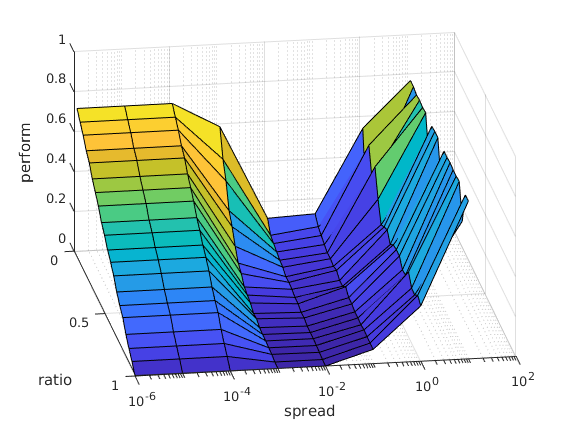
\includegraphics[scale=0.8]{4_5}
	\caption{Зависимость \code{perform} от \code{spread} и \code{ratio}}
	\label{fig:4_5}
\end{center}
\end{figure}
Из графика видно, что ошибка возрастает при уменьшении объема обучающей выборки, при этом приемлемыми значениями параметра \code{spread} являются $10^{-4} \div 10^{-2}$.

По сравнению с сетями прямого распространения, PNN смогла добиться нулевой ошибки, в то время как НСПР лишь $\sim 0.5$. Однако, в PNN количество нейронов равняется обучающей выборке ($1681$ нейрон), в то время как в НСПР требовалось около $30$ нейронов для данной классификации. PNN оказалось проще настроить, так как необходимо задать только один параметр \code{spread}. В НСПР же необходимо задавать количество нейронов скрытого слоя и пар метры функции обучения.

\newpage

\section{Классификация многомерных образов}

\subsection{Формирование обучающей и тестовой выборки}

%Сформируйте обучающую выборку достаточного объема.

Сформируем обучающую и тестовую выборки на основе ранее созданных функций. Объем выборки составляет 1797 примеров. На рис. \ref{fig:5_1_1} изображены примеры обучающей выборки.
\begin{figure}[H]
\begin{center}
	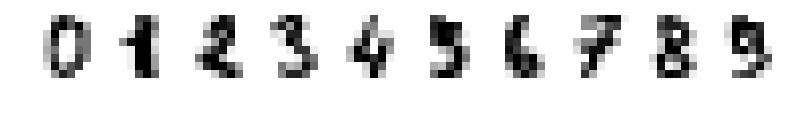
\includegraphics[scale=1]{5_1_1}
	\caption{Исходные образы \code{P}}
	\label{fig:5_1_1}
\end{center}
\end{figure}

Сформируем зашумленные образы, повернутые на случайный угол и сдвинутые относительно исходных. На рис. \ref{fig:5_1_2} изображены примеры таких образов.
\begin{figure}[H]
\begin{center}
	\begin{subfigure}[b]{\textwidth}
		
\includegraphics[scale=1]{5_1_2}
		\caption{Зашумленная выборка \code{P_noisy}}
	\end{subfigure}
	\begin{subfigure}[b]{\textwidth}
		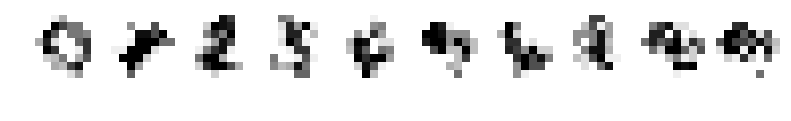
\includegraphics[scale=1]{5_1_3}
		\caption{Повернутая выборка \code{P_rotate}}
	\end{subfigure}
	\begin{subfigure}[b]{\textwidth}
		
\includegraphics[scale=1]{5_1_4}
		\caption{Сдвинутая выборка \code{P_shift}}
	\end{subfigure}
	\caption{Примеры разбиений}
	\label{fig:5_1_2}
\end{center}
\end{figure}

\subsection{Подбор значения spread}

%Подберите оптимальное значение spread.

На рис. \ref{fig:5_2_1} приведена зависимость ошибки \code{perform} от значения параметра \code{spread} в логарифмическом масштабе. 
\vspace{-0.5cm}
\begin{figure}[H]
\begin{center}
	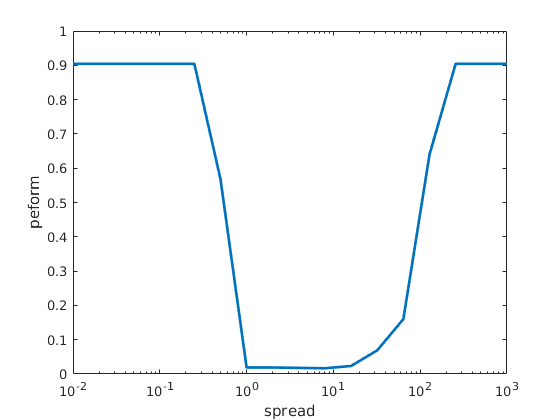
\includegraphics[scale=0.75]{5_2_1}
	\caption{Зависимость \code{perform} от \code{spread}}
	\label{fig:5_2_1}
\end{center}
\end{figure}
\vspace{-1cm}

Оптимальным можно также считать \code{spread = 10}. На рис. \ref{fig:5_2_2} приведена матрица неточностей тестовой выборки при \code{spread = 10}.
\vspace{-0.5cm}
\begin{figure}[H]
\begin{center}
	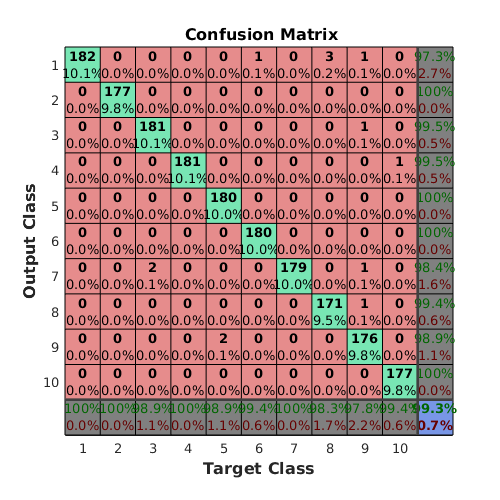
\includegraphics[scale=0.8]{5_2_2}
	\caption{Матрица неточностей, err = 0.0072}
	\label{fig:5_2_2}
\end{center}
\end{figure}

\subsection{Качество классификации}

%Исследуйте качество классификации на тестовой выборке, содержащей зашумленные примеры. Приведите матрицу неточностей, рассчитайте среднюю ошибку и ошибки 1,2 родов.

Исследуем качество классификации на зашумленные образах, образах, повернутых на случайный угол, и образах, сдвинутых относительно исходных. На рис. \ref{fig:5_3_1} - \ref{fig:5_3_3} изображены матрицы неточностей для искаженных входных образов.
\begin{figure}[H]
\begin{center}
	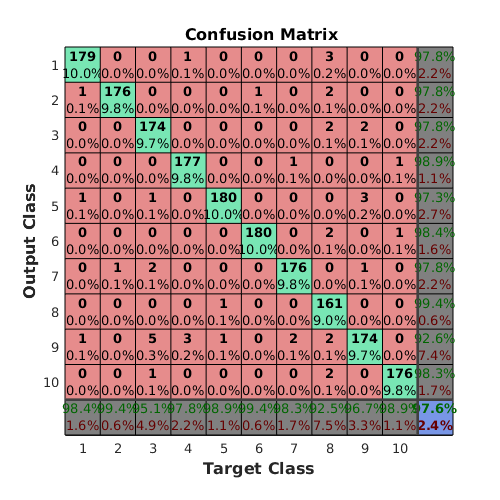
\includegraphics[scale=0.8]{5_3_1}
	\caption{Матрицы неточностей для \code{P_noisy}, err = 0.0245}
	\label{fig:5_3_1}
\end{center}
\end{figure}
Ошибки 1 и 2 рода соответственно равны:
\begin{gather*}
e_1 = [0.0219, 0.0222, 0.0225, 0.0112, 0.0270, 0.0164, 0.0222, 0.0062, 0.0745, 0.0168]\\
e_2 = [0.0165, 0.0056, 0.0492, 0.0221, 0.0110, 0.0055, 0.0168, 0.0747, 0.0333, 0.0112]
\end{gather*}

\begin{figure}[H]
\begin{center}
	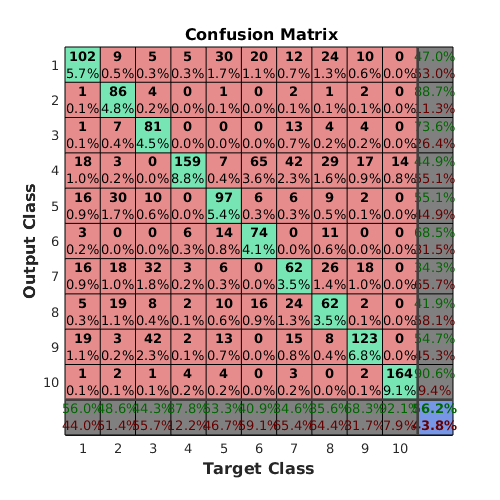
\includegraphics[scale=0.8]{5_3_2}
	\caption{Матрицы неточностей для \code{P_rotate}, err = 0.4380}
	\label{fig:5_3_2}
\end{center}
\end{figure}
Ошибки 1 и 2 рода соответственно равны:
\begin{gather*}
e_1 = [0.5300, 0.1134, 0.2636, 0.5508, 0.4489, 0.3148, 0.6575, 0.5811, 0.4533, 0.0939]\\
e_2 = [0.4396, 0.5141, 0.5574, 0.1215, 0.4670, 0.5912, 0.6536, 0.6437, 0.3167, 0.0787]
\end{gather*}

\begin{figure}[H]
\begin{center}
	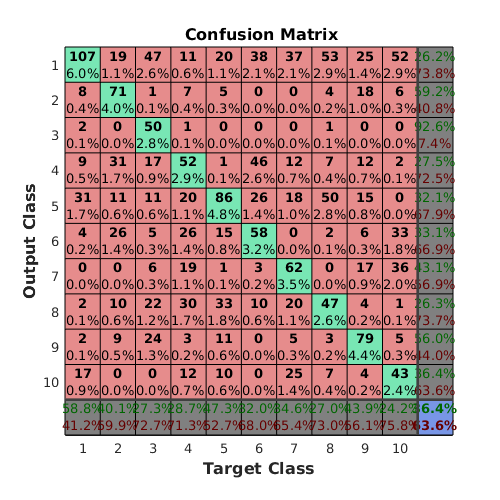
\includegraphics[scale=0.8]{5_3_3}
	\caption{Матрицы неточностей для \code{P_shift}, err = 0.6355}
	\label{fig:5_3_3}
\end{center}
\end{figure}
Ошибки 1 и 2 рода соответственно равны:
\begin{gather*}
e_1 = [0.7384, 0.4083, 0.0741, 0.7249, 0.6791, 0.6686, 0.5694, 0.7374, 0.4397, 0.6356]\\
e_2 = [0.4121, 0.5989, 0.7268, 0.7127, 0.5275, 0.6796, 0.6536, 0.7299, 0.5611, 0.7584]
\end{gather*}

\newpage

\subsection{Изменение объема выборки}

%Попробуйте увеличить и уменьшить объем обучающей выборки в несколько раз. Для каждого случая подберите оптимальное значение spread и рассчитайте показатели качества классификации.
%Проанализируйте полученные результаты, сравнив их с результатами классификации тех же самых образов НС прямого распространения по аналогии с п. 3 задания 1.

Построим зависимость ошибки \code{perform} от параметра \code{spread} и объема обучающей выборки \code{ratio} (если \code{ratio = 1}, то обучение на всей выборке). 
\begin{figure}[H]
\begin{center}
	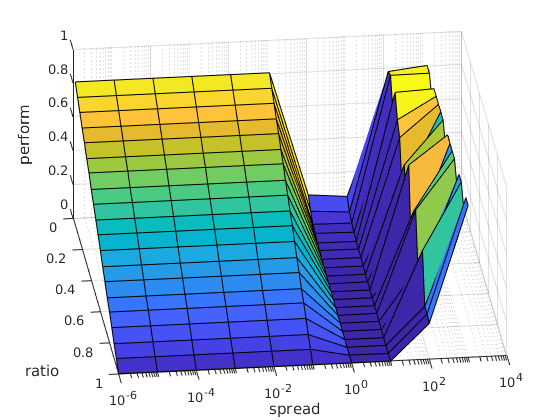
\includegraphics[scale=0.8]{5_4_1}
	\caption{Зависимость \code{perform} от \code{spread} и \code{ratio}}
	\label{fig:5_4_1}
\end{center}
\end{figure}
Из графика видно, что ошибка возрастает при уменьшении объема обучающей выборки, при этом приемлемыми значениями параметра \code{spread} являются $1 \div 10$.

Уменьшим обучающую выборку сначала в 5 раз, т.е. с 1797 примера до 358, а затем в 10 раз, т.е. с 1797 примера до 179. На рис. \ref{fig:5_4_2} приведены получаемые матрицы неточностей.
\begin{figure}[H]
\begin{center}
	\begin{subfigure}{0.49\textwidth}
		\includegraphics[width=\textwidth]{5_4_2}
		\caption{\code{ratio = 0.2}, err = 0.0295}
	\end{subfigure}
	\begin{subfigure}{0.49\textwidth}
		\includegraphics[width=\textwidth]{5_4_3}
		\caption{\code{ratio = 0.1}, err = 0.0523}
	\end{subfigure}
	\caption{Матрицы неточностей при разных объемах выборки}
	\label{fig:5_4_2}
\end{center}
\end{figure}

По сравнению с сетями прямого распространения, PNN смогла добиться ошибки на тестовой выборке, близкой к нулевой, в то время как НСПР лишь $\sim 0.1$. Однако, в PNN количество нейронов равняется обучающей выборке ($899$ нейрон), в то время как в НСПР требовалось около $100$ нейронов для данной классификации. PNN оказалось проще настроить, так как необходимо задать только один параметр \code{spread}. В НСПР же необходимо задавать количество нейронов скрытого слоя и пар метры функции обучения.

\section{Выводы}

В данной работе были приобретены навыки построения, инициализации и обучения нейронных сетей с радиально-базисными функциями для решения задач аппроксимации статической аппроксимации и классификации. Были изучены точные РБФ-НС, приближенные РБФ-НС и GRNN.

\end{document}